% answers.tex —— 2011 年·全国大纲卷·文科 · 参考答案与详细解析片段
% 由 tools/generate_projects.py 依来源总账自 2011/2011_数学真题_全国大纲文_试题.md + 2011/2011_数学真题_全国大纲文_解析正文.md + 2011/2011_数学真题_全国大纲文_答案要点.md 生成，勿手改（改源 MD 后重跑）


\begin{answer}
\gksolhead{1}{}

\textbf{题目}：

设集合 $U=\{1,2,3,4\}$，$M=\{1,2,3\}$，$N=\{2,3,4\}$，则 $\complement_U(M\cap N)=$\mbox{（　　）}

（A）$\{1,2\}$\quad（B）$\{2,3\}$\quad（C）$\{2,4\}$\quad（D）$\{1,4\}$

\Needspace{4\baselineskip}
\textbf{解析}

$M\cap N=\{2,3\}$，所以
$\complement_U(M\cap N)=\{1,4\}$，选 D。

\gkanswer{答案：D}

\end{answer}
\begin{answer}
\gksolhead{2}{}

\textbf{题目}：

函数 $y=2\sqrt{x}$（$x\geq0$）的反函数为\mbox{（　　）}

（A）$y=\dfrac{x^2}{4}$（$x\in\mathbb R$）\quad（B）$y=\dfrac{x^2}{4}$（$x\geq0$）

（C）$y=4x^2$（$x\in\mathbb R$）\quad（D）$y=4x^2$（$x\geq0$）

\Needspace{4\baselineskip}
\textbf{解析}

由 $y=2\sqrt{x}$ 交换 $x\text{、}y$，得
$x=2\sqrt{y}$，从而 $y=x^2/4$，且反函数的定义域为 $x\geq0$，选 B。

\gkanswer{答案：B}

\end{answer}
\begin{answer}
\gksolhead{3}{}

\textbf{题目}：

设向量 $\boldsymbol a\text{、}\boldsymbol b$ 满足 $|\boldsymbol a|=|\boldsymbol b|=1$，$\boldsymbol a\cdot\boldsymbol b=-\dfrac12$，则 $|\boldsymbol a+2\boldsymbol b|=$\mbox{（　　）}

（A）$\sqrt2$\quad（B）$\sqrt3$\quad（C）$\sqrt5$\quad（D）$\sqrt7$

\Needspace{4\baselineskip}
\textbf{解析}

\nopagebreak[4]
\[
|\boldsymbol a+2\boldsymbol b|^2
=|\boldsymbol a|^2+4|\boldsymbol b|^2+4\boldsymbol a\cdot\boldsymbol b
=1+4-2=3.
\]

故 $|\boldsymbol a+2\boldsymbol b|=\sqrt3$，选 B。

\gkanswer{答案：B}

\end{answer}
\begin{answer}
\gksolhead{4}{}

\textbf{题目}：

\Needspace{5\baselineskip}
若变量 $x\text{、}y$ 满足约束条件

\nopagebreak[4]
\[
\begin{cases}
x+y\leq6,\\
x-3y\leq-2,\\
x\geq1,
\end{cases}
\]

则 $z=2x+3y$ 的最小值为\mbox{（　　）}

（A）$17$\quad（B）$14$\quad（C）$5$\quad（D）$3$

\Needspace{4\baselineskip}
\textbf{解析}

\Needspace{5\baselineskip}
由 $x-3y\leq-2$ 得 $y\geq(x+2)/3$，于是
\nopagebreak[4]
\[
z=2x+3y\geq2x+x+2=3x+2\geq5.
\]
当 $(x,y)=(1,1)$ 时等号成立，选 C。

\gkanswer{答案：C}

\end{answer}
\begin{answer}
\gksolhead{5}{}

\textbf{题目}：

下面四个条件中，使 $a>b$ 成立的充分而不必要的条件是\mbox{（　　）}

（A）$a>b+1$\quad（B）$a>b-1$\quad（C）$a^2>b^2$\quad（D）$a^3>b^3$

\Needspace{4\baselineskip}
\textbf{解析}

$a>b+1$ 必然推出 $a>b$，但 $a>b$ 不必推出 $a>b+1$，所以它是充分而不必要条件，选 A。

\gkanswer{答案：A}

\end{answer}
\begin{answer}
\gksolhead{6}{}

\textbf{题目}：

设 $S_n$ 为等差数列 $\{a_n\}$ 的前 $n$ 项和，若 $a_1=1$，公差 $d=2$，$S_{k+2}-S_k=24$，则 $k=$\mbox{（　　）}

（A）$8$\quad（B）$7$\quad（C）$6$\quad（D）$5$

\Needspace{4\baselineskip}
\textbf{解析}

\Needspace{5\baselineskip}
等差数列的通项为 $a_n=1+2(n-1)=2n-1$，所以
\nopagebreak[4]
\[
S_{k+2}-S_k=a_{k+1}+a_{k+2}
=(2k+1)+(2k+3)=4k+4.
\]

由 $4k+4=24$ 得 $k=5$，选 D。

\gkanswer{答案：D}

\end{answer}
\begin{answer}
\gksolhead{7}{}

\textbf{题目}：

设函数 $f(x)=\cos\omega x$（$\omega>0$），将 $y=f(x)$ 的图象向右平移 $\dfrac\pi3$ 个单位长度后，所得的图象与原图象重合，则 $\omega$ 的最小值等于\mbox{（　　）}

（A）$\dfrac13$\quad（B）$3$\quad（C）$6$\quad（D）$9$

\Needspace{4\baselineskip}
\textbf{解析}

平移后图象重合说明 $\pi/3$ 是函数的一个周期。因周期为
\Needspace{5\baselineskip}
$2\pi/\omega$，有
\nopagebreak[4]
\[
\frac{\pi}{3}=m\frac{2\pi}{\omega}\quad(m\in\mathbb N^+).
\]

故 $\omega=6m$，最小值为 $6$，选 C。

\gkanswer{答案：C}

\end{answer}
\begin{answer}
\gksolhead{8}{}

\textbf{题目}：

已知直二面角 $\alpha-l-\beta$，点 $A\in\alpha$，$AC\perp l$，$C$ 为垂足，点 $B\in\beta$，$BD\perp l$，$D$ 为垂足。若 $AB=2$，$AC=BD=1$，则 $CD=$\mbox{（　　）}

（A）$2$\quad（B）$\sqrt3$\quad（C）$\sqrt2$\quad（D）$1$

\Needspace{4\baselineskip}
\textbf{解析}

取公共棱 $l$ 为 $x$ 轴，令
$C=(0,0,0)$、$D=(d,0,0)$。两侧面互相垂直，可取
\Needspace{5\baselineskip}
$A=(0,1,0)$、$B=(d,0,1)$。于是
\nopagebreak[4]
\[
AB^2=CD^2+AC^2+BD^2=d^2+2.
\]

由 $AB=2$ 得 $d^2=2$，所以 $CD=\sqrt2$，选 C。

\gkanswer{答案：C}

\end{answer}
\begin{answer}
\gksolhead{9}{}

\textbf{题目}：

$4$ 位同学每人从甲、乙、丙 $3$ 门课程中选修 $1$ 门，则恰有 $2$ 人选修课程甲的不同选法共有\mbox{（　　）}

（A）$12$ 种\quad（B）$24$ 种\quad（C）$30$ 种\quad（D）$36$ 种

\Needspace{4\baselineskip}
\textbf{解析}

\Needspace{5\baselineskip}
先从 $4$ 位同学中选出恰好选甲的 $2$ 位，再令另外 $2$ 位各自从乙、丙中选择，方法数为
\nopagebreak[4]
\[
\binom42\cdot2^2=24.
\]

选 B。

\gkanswer{答案：B}

\end{answer}
\begin{answer}
\gksolhead{10}{}

\textbf{题目}：

设 $f(x)$ 是周期为 $2$ 的奇函数，当 $0\leq x\leq1$ 时，$f(x)=2x(1-x)$，则 $f\left(-\dfrac52\right)=$\mbox{（　　）}

（A）$-\dfrac12$\quad（B）$-\dfrac14$\quad（C）$\dfrac14$\quad（D）$\dfrac12$

\Needspace{4\baselineskip}
\textbf{解析}

\Needspace{5\baselineskip}
利用周期性和奇偶性，
\nopagebreak[4]
\[
f\left(-\frac52\right)=f\left(-\frac12\right)
=-f\left(\frac12\right)
=-(2\cdot\tfrac12\cdot\tfrac12)=-\frac12.
\]

选 A。

\gkanswer{答案：A}

\end{answer}
\begin{answer}
\gksolhead{11}{}

\textbf{题目}：

设两圆 $C_1\text{、}C_2$ 都和两坐标轴相切，且都过点 $(4,1)$，则两圆心的距离 $|C_1C_2|=$\mbox{（　　）}

（A）$4$\quad（B）$4\sqrt2$\quad（C）$8$\quad（D）$8\sqrt2$

\Needspace{4\baselineskip}
\textbf{解析}

\Needspace{5\baselineskip}
设圆心在第一象限的圆半径为 $r$，圆心为 $(r,r)$。代入点 $(4,1)$ 得
\nopagebreak[4]
\[
(4-r)^2+(1-r)^2=r^2,
\]
即 $r^2-10r+17=0$，所以两个半径为
\Needspace{5\baselineskip}
$r_1=5+2\sqrt2$、$r_2=5-2\sqrt2$。两圆心均在直线 $y=x$ 上，故
\nopagebreak[4]
\[
|C_1C_2|=\sqrt2\,|r_1-r_2|=8.
\]

选 C。

\gkanswer{答案：C}

\end{answer}
\begin{answer}
\gksolhead{12}{}

\textbf{题目}：

已知平面 $\alpha$ 截一球面得圆 $M$，过圆心 $M$ 且与 $\alpha$ 成 $60^\circ$ 二面角的平面 $\beta$ 截该球面得圆 $N$。若该球面的半径为 $4$，圆 $M$ 的面积为 $4\pi$，则圆 $N$ 的面积为\mbox{（　　）}

（A）$7\pi$\quad（B）$9\pi$\quad（C）$11\pi$\quad（D）$13\pi$

\Needspace{4\baselineskip}
\textbf{解析}

球半径为 $4$，圆 $M$ 的半径为 $2$，所以球心到平面
\Needspace{5\baselineskip}
$\alpha$ 的距离为
\nopagebreak[4]
\[
d_\alpha=\sqrt{4^2-2^2}=2\sqrt3.
\]

\Needspace{5\baselineskip}
平面 $\beta$ 经过 $M$，且与 $\alpha$ 成 $60^\circ$ 二面角。两平面的法向量也成 $60^\circ$，故球心到 $\beta$ 的距离为
\nopagebreak[4]
\[
d_\beta=d_\alpha\cos60^\circ=\sqrt3.
\]

于是圆 $N$ 的半径平方为 $4^2-d_\beta^2=13$，面积为 $13\pi$，选 D。

\gkanswer{答案：D}

\end{answer}
\begin{answer}
\gksolhead{13}{}

\textbf{题目}：

$(1-x)^{10}$ 的二项展开式中，$x$ 的系数与 $x^9$ 的系数之差为\gkblank{}。

\Needspace{4\baselineskip}
\textbf{解析}

$(1-x)^{10}$ 中 $x$ 的系数为 $-\binom{10}{1}=-10$，$x^9$ 的系数为
$(-1)^9\binom{10}{9}=-10$，两者之差为 $0$。

\gkanswer{答案：$0$}

\end{answer}
\begin{answer}
\gksolhead{14}{}

\textbf{题目}：

已知 $\alpha\in\left(\pi,\dfrac{3\pi}{2}\right)$，$\tan\alpha=2$，则 $\cos\alpha=$\gkblank{}。

\Needspace{4\baselineskip}
\textbf{解析}

\Needspace{5\baselineskip}
$\alpha$ 在第三象限，且 $\tan\alpha=2$，由三角函数基本关系得
\nopagebreak[4]
\[
\cos\alpha=-\frac1{\sqrt{1+\tan^2\alpha}}
=-\frac1{\sqrt5}.
\]

\gkanswer{答案：$-\dfrac1{\sqrt5}$}

\end{answer}
\begin{answer}
\gksolhead{15}{}

\textbf{题目}：

已知正方体 $ABCD-A_1B_1C_1D_1$ 中，$E$ 为 $C_1D_1$ 的中点，则异面直线 $AE$ 与 $BC$ 所成角的余弦值为\gkblank{}。

\Needspace{4\baselineskip}
\textbf{解析}

设正方体棱长为 $1$，取
$A=(0,0,0)$、$B=(1,0,0)$、$C=(1,1,0)$、$D=(0,1,0)$，则
\Needspace{5\baselineskip}
$E=(1/2,1,1)$。于是
\nopagebreak[4]
\[
\overrightarrow{AE}=\left(\frac12,1,1\right),\qquad
\overrightarrow{BC}=(0,1,0),
\]
\Needspace{5\baselineskip}
从而
\nopagebreak[4]
\[
\cos\angle(AE,BC)
=\frac{\overrightarrow{AE}\cdot\overrightarrow{BC}}
{|\overrightarrow{AE}|\,|\overrightarrow{BC}|}
=\frac1{\sqrt{1/4+1+1}}=\frac23.
\]

\gkanswer{答案：$\dfrac23$}

\end{answer}
\begin{answer}
\gksolhead{16}{}

\textbf{题目}：

已知 $F_1\text{、}F_2$ 分别为双曲线 $C:\dfrac{x^2}{9}-\dfrac{y^2}{27}=1$ 的左、右焦点，点 $A\in C$，点 $M$ 的坐标为 $(2,0)$，$AM$ 为 $\angle F_1AF_2$ 的平分线，则 $|AF_2|=$\gkblank{}。

\Needspace{4\baselineskip}
\textbf{解析}

双曲线的半长轴为 $3$，焦距参数为
$c=\sqrt{3^2+27}=6$，故
$F_1=(-6,0)$、$F_2=(6,0)$。点 $M=(2,0)$ 位于
\Needspace{5\baselineskip}
$F_1F_2$ 上，且
\nopagebreak[4]
\[
F_1M:MF_2=8:4=2:1.
\]

由角平分线定理，
$AF_1:AF_2=2:1$。又双曲线右支满足
$AF_1-AF_2=2a=6$，所以 $AF_2=6$。

\gkanswer{答案：$6$}

\end{answer}
\begin{answer}
\gksolhead{17}{}

\textbf{题目}：

设等比数列 $\{a_n\}$ 的前 $n$ 项和为 $S_n$，已知 $a_2=6$，$6a_1+a_3=30$，求 $a_n$ 和 $S_n$。

\Needspace{4\baselineskip}
\textbf{解析}

设公比为 $q$。由 $a_2=6$，有
\Needspace{5\baselineskip}
$a_1=6/q$、$a_3=6q$，代入
\nopagebreak[4]
\[
6a_1+a_3=30
\]
\Needspace{5\baselineskip}
得
\nopagebreak[4]
\[
\frac{36}{q}+6q=30,\qquad q^2-5q+6=0.
\]

\Needspace{5\baselineskip}
因此 $q=2$ 或 $q=3$。相应地，
\nopagebreak[4]
\[
q=2:\quad a_n=3\cdot2^{n-1},\qquad
S_n=3(2^n-1);
\]
\nopagebreak[4]
\[
q=3:\quad a_n=2\cdot3^{n-1},\qquad
S_n=3^n-1.
\]

\gkanswer{答案：有两组解：$(a_n,S_n)=\left(2\cdot3^{n-1},\,3^n-1\right)$ 或 $(a_n,S_n)=\left(3\cdot2^{n-1},\,3(2^n-1)\right)$。}

\end{answer}
\begin{answer}
\gksolhead{18}{}

\textbf{题目}：

\Needspace{5\baselineskip}
$\triangle ABC$ 的内角 $A\text{、}B\text{、}C$ 的对边分别为 $a\text{、}b\text{、}c$。已知

\nopagebreak[4]
\[
a\sin A+c\sin C-\sqrt2a\sin C=b\sin B.
\]

（1） 求 $B$；

（2） 若 $A=75^\circ$，$b=2$，求 $a\text{、}c$。

\Needspace{4\baselineskip}
\textbf{解析}

\gksubpart{(1)}

由正弦定理设 $a=K\sin A$、$b=K\sin B$、
\Needspace{5\baselineskip}
$c=K\sin C$。原式化为
\nopagebreak[4]
\[
\sin^2A+\sin^2C-\sqrt2\sin A\sin C=\sin^2B.
\]

\Needspace{5\baselineskip}
利用
\nopagebreak[4]
\[
\sin^2A+\sin^2C=1-\cos(A+C)\cos(A-C),
\qquad
\sin A\sin C=\frac{\cos(A-C)-\cos(A+C)}2
\]
\Needspace{5\baselineskip}
以及 $A+B+C=\pi$，可得
\nopagebreak[4]
\[
\left(\cos B-\frac{\sqrt2}{2}\right)
\left(\cos B+\cos(A-C)\right)=0.
\]

\Needspace{5\baselineskip}
又
\nopagebreak[4]
\[
\cos B+\cos(A-C)=2\sin A\sin C>0,
\]
所以 $\cos B=\sqrt2/2$，即 $B=45^\circ$。

\gksubpart{(2)}

\Needspace{5\baselineskip}
当 $A=75^\circ$ 时，$C=60^\circ$。由正弦定理且 $b=2$，
\nopagebreak[4]
\[
a=\frac{2\sin75^\circ}{\sin45^\circ}=1+\sqrt3,
\qquad
c=\frac{2\sin60^\circ}{\sin45^\circ}=\sqrt6.
\]

\gkanswer{答案（1）：$B=45^\circ$。}

\gkanswer{答案（2）：$a=1+\sqrt3$，$c=\sqrt6$。}

\end{answer}
\begin{answer}
\gksolhead{19}{}

\textbf{题目}：

根据以往统计资料，某地车主购买甲种保险的概率为 $0.5$，购买乙种保险但不购买甲种保险的概率为 $0.3$。设各车主购买保险相互独立。

（1） 求该地 $1$ 位车主至少购买甲、乙两种保险中的 $1$ 种的概率；

（2） 求该地 $3$ 位车主中恰有 $1$ 位车主甲、乙两种保险都不购买的概率。

\Needspace{4\baselineskip}
\textbf{解析}

\gksubpart{(1)}

不购买甲保险的概率为 $1-0.5=0.5$，其中不购买甲而购买乙的概率为
\Needspace{5\baselineskip}
$0.3$，所以两种保险都不购买的概率为
\nopagebreak[4]
\[
0.5-0.3=0.2.
\]

\gksubpart{(2)}

（1）至少购买一种保险的概率为 $1-0.2=0.8$。

\Needspace{5\baselineskip}
（2）三位车主中恰有一位两种保险都不购买的概率为
\nopagebreak[4]
\[
\binom31(0.2)(0.8)^2=0.384=\frac{48}{125}.
\]

\gkanswer{答案（1）：至少购买一种保险的概率为 $0.8$。}

\gkanswer{答案（2）：恰有 $1$ 位车主两种保险都不购买的概率为 $\binom31(0.2)(0.8)^2=0.384=\dfrac{48}{125}$。}

\end{answer}
\begin{answer}
\gksolhead{20}{}

\textbf{题目}：

如图，四棱锥 $S-ABCD$ 中，$AB\parallel CD$，$BC\perp CD$，侧面 $SAB$ 为等边三角形。$AB=BC=2$，$CD=SD=1$。
\nopagebreak[4]
\begin{center}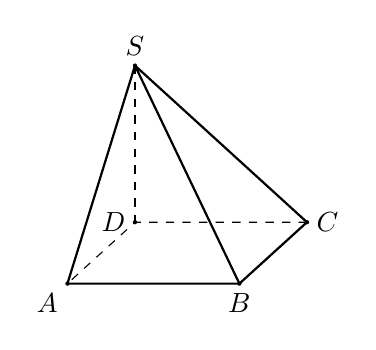
\begin{tikzpicture}[scale=.78,>=stealth]
\coordinate (A) at (0,0);
\coordinate (B) at (2.8,0);
\coordinate (C) at (3.9,1.0);
\coordinate (D) at (1.1,1.0);
\coordinate (S) at (1.1,3.55);
\draw[thick] (A)--(B)--(C);
\draw[dashed] (C)--(D)--(A);
\draw[thick] (S)--(A) (S)--(B) (S)--(C);
\draw[dashed] (S)--(D);
\fill (A) circle (1pt) node[below left] {$A$};
\fill (B) circle (1pt) node[below] {$B$};
\fill (C) circle (1pt) node[right] {$C$};
\fill (D) circle (1pt) node[left] {$D$};
\fill (S) circle (1pt) node[above] {$S$};
\end{tikzpicture}
\end{center}
\nopagebreak[4]
（1） 证明：$SD\perp$ 平面 $SAB$；

（2） 求 $AB$ 与平面 $SBC$ 所成角的大小。

\Needspace{4\baselineskip}
\textbf{解析}

\gksubpart{(1)}

\Needspace{5\baselineskip}
建立直角坐标系，取
\nopagebreak[4]
\[
A=(0,0,0),\quad B=(2,0,0),\quad
C=(2,2,0),\quad D=(1,2,0).
\]
\Needspace{5\baselineskip}
设 $S=(1,u,v)$。由 $SAB$ 为边长 $2$ 的等边三角形，
\nopagebreak[4]
\[
u^2+v^2=3.
\]
\Needspace{5\baselineskip}
再由 $SD=1$，得
\nopagebreak[4]
\[
(u-2)^2+v^2=1,
\]
所以 $u=3/2$、$v=\sqrt3/2$。

\Needspace{5\baselineskip}
于是
\nopagebreak[4]
\[
\overrightarrow{SD}=\left(0,\frac12,-\frac{\sqrt3}{2}\right),
\quad
\overrightarrow{AB}=(2,0,0),
\quad
\overrightarrow{AS}=\left(1,\frac32,\frac{\sqrt3}{2}\right).
\]

有 $\overrightarrow{SD}\cdot\overrightarrow{AB}=0$ 且
$\overrightarrow{SD}\cdot\overrightarrow{AS}=0$，故
$SD\perp$ 平面 $SAB$。

\gksubpart{(2)}

\Needspace{5\baselineskip}
取平面 $SBC$ 的一个法向量
\nopagebreak[4]
\[
\boldsymbol n=(\sqrt3,0,2),\qquad |\boldsymbol n|=\sqrt7.
\]
\Needspace{5\baselineskip}
设 $AB$ 与平面 $SBC$ 所成角为 $\theta$，则
\nopagebreak[4]
\[
\sin\theta
=\frac{|\overrightarrow{AB}\cdot\boldsymbol n|}
{|\overrightarrow{AB}|\,|\boldsymbol n|}
=\frac{\sqrt3}{\sqrt7}.
\]

\gkanswer{答案（1）：见解析版}

\gkanswer{答案（2）：$AB$ 与平面 $SBC$ 所成角的大小满足 $\sin\theta=\dfrac{\sqrt3}{\sqrt7}=\dfrac{\sqrt{21}}7$，即 $\theta=\arcsin\dfrac{\sqrt{21}}7$。}

\end{answer}
\begin{answer}
\gksolhead{21}{}

\textbf{题目}：

已知函数 $f(x)=x^3+3ax^2+(3-6a)x+12a-4$（$a\in\mathbb R$）。

（1） 证明：曲线 $y=f(x)$ 在 $x=0$ 处的切线过点 $(2,2)$；

（2） 若 $f(x)$ 在 $x=x_0$ 处取得极小值，$x_0\in(1,3)$，求 $a$ 的取值范围。

\Needspace{4\baselineskip}
\textbf{解析}

\gksubpart{(1)}

\Needspace{5\baselineskip}
有
\nopagebreak[4]
\[
f(0)=12a-4,\qquad f'(0)=3-6a.
\]
\Needspace{5\baselineskip}
故曲线在 $x=0$ 处的切线为
\nopagebreak[4]
\[
y=(3-6a)x+12a-4.
\]
将 $x=2$ 代入，右端恒为 $2$，所以切线恒过 $(2,2)$。

\gksubpart{(2)}

\Needspace{5\baselineskip}
又
\nopagebreak[4]
\[
f'(x)=3\left[x^2+2ax+1-2a\right].
\]
\Needspace{5\baselineskip}
若极小值点为 $x_0\in(1,3)$，则 $f'(x_0)=0$，从而
\nopagebreak[4]
\[
a=-\frac{x_0^2+1}{2(x_0-1)}.
\]
\Needspace{5\baselineskip}
极小值还要求
\nopagebreak[4]
\[
f''(x_0)=6(x_0+a)>0.
\]
代入上式后等价于 $x_0>1+\sqrt2$。因此
\Needspace{5\baselineskip}
$x_0\in(1+\sqrt2,3)$。函数
\nopagebreak[4]
\[
h(x)=-\frac{x^2+1}{2(x-1)}
\]
\Needspace{5\baselineskip}
在该区间上递减，且
\nopagebreak[4]
\[
\lim_{x\to(1+\sqrt2)^+}h(x)=-1-\sqrt2,\qquad
\lim_{x\to3^-}h(x)=-\frac52.
\]
\Needspace{5\baselineskip}
所以
\nopagebreak[4]
\[
a\in\left(-\frac52,-1-\sqrt2\right).
\]

\gkanswer{答案（1）：切线为 $y=(3-6a)x+12a-4$。}

\gkanswer{答案（2）：$a\in\left(-\dfrac52,-1-\sqrt2\right)$。}

\end{answer}
\begin{answer}
\gksolhead{22}{}

\textbf{题目}：

\Needspace{5\baselineskip}
已知 $O$ 为坐标原点，$F$ 为椭圆 $C:x^2+\dfrac{y^2}{2}=1$ 在 $y$ 轴正半轴上的焦点，过 $F$ 且斜率为 $-\sqrt2$ 的直线 $l$ 与 $C$ 交于 $A\text{、}B$ 两点，点 $P$ 满足

\nopagebreak[4]
\[
\overrightarrow{OA}+\overrightarrow{OB}+\overrightarrow{OP}=\boldsymbol0.
\]
\nopagebreak[4]
\begin{center}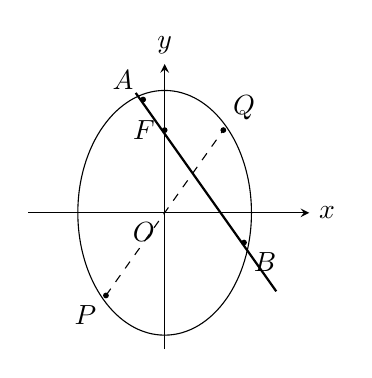
\begin{tikzpicture}[>=stealth,scale=1.05]
\draw[->] (-1.65,0)--(1.75,0) node[right] {$x$};
\draw[->] (0,-1.65)--(0,1.8) node[above] {$y$};
\draw (0,0) ellipse [x radius=1.05,y radius=1.48];
\draw[thick] (-.35,1.45)--(1.35,-.95);
\fill (-.26,1.37) circle (1pt) node[above left] {$A$};
\fill (.96,-.36) circle (1pt) node[below right] {$B$};
\fill (0,1) circle (1pt) node[left] {$F$};
\fill (-.71,-1) circle (1pt) node[below left] {$P$};
\fill (.71,1) circle (1pt) node[above right] {$Q$};
\draw[dashed] (-.71,-1)--(.71,1);
\node[below left] at (0,0) {$O$};
\end{tikzpicture}
\end{center}
\nopagebreak[4]
（1） 证明：点 $P$ 在 $C$ 上；

（2） 设点 $P$ 关于点 $O$ 的对称点为 $Q$，证明：$A\text{、}P\text{、}B\text{、}Q$ 四点在同一圆上。

\Needspace{4\baselineskip}
\textbf{解析}

\gksubpart{(1)}

\Needspace{5\baselineskip}
由韦达定理，
\nopagebreak[4]
\[
AD\cdot AB=mn=AE\cdot AC.
\]
由于 $D\in AB$、$E\in AC$，这正是从点 $A$ 引出的两条割线满足的乘积相等条件。由相交弦定理的逆定理，$C\text{、}B\text{、}D\text{、}E$ 四点共圆。

\gksubpart{(2)}

\Needspace{5\baselineskip}
当 $m=4,n=6$ 时，方程
\nopagebreak[4]
\[
x^2-14x+24=0
\]
的两根为 $2$、$12$。因 $D$、$E$ 不与顶点重合且在边上，取
\Needspace{5\baselineskip}
$AD=2$、$AB=12$、$AE=4$、$AC=6$。令
\nopagebreak[4]
\[
A=(0,0),\quad B=(12,0),\quad C=(0,6),\quad
D=(2,0),\quad E=(0,4).
\]

\Needspace{5\baselineskip}
所在圆方程为
\nopagebreak[4]
\[
x^2+y^2-14x-10y+24=0,
\]
\Needspace{5\baselineskip}
故圆心为 $(7,5)$，半径为
\nopagebreak[4]
\[
\sqrt{7^2+5^2-24}=5\sqrt2.
\]

\gkanswer{答案（1）：见解析版}

\gkanswer{答案（2）：见解析版}

\end{answer}